% THIS DOCUMENT IS TAILORED TO REQUIREMENTS FOR SCIENTIFIC COMPUTING.  IT SHOULDN'T
% BE USED FOR NON-SCIENTIFIC COMPUTING PROJECTS
\documentclass[12pt]{article}

\usepackage{amsmath, mathtools}
\usepackage{amsfonts}
\usepackage{amssymb}
\usepackage{graphicx}
\usepackage{colortbl}
\usepackage{xr}
\usepackage{hyperref}
\usepackage{longtable}
\usepackage{xfrac}
\usepackage{tabularx}
\usepackage{float}
\usepackage{siunitx}
\usepackage{booktabs}
\usepackage{caption}
\usepackage{pdflscape}
\usepackage{afterpage}

\usepackage[round]{natbib}

%\usepackage{refcheck}

\hypersetup{
    colorlinks=true,       % false: boxed links; true: colored links
    linkcolor=red,          % color of internal links (change box color with linkbordercolor)
    citecolor=green,        % color of links to bibliography
    filecolor=magenta,      % color of file links
    urlcolor=cyan           % color of external links
}

%% Comments

\usepackage{color}

\newif\ifcomments\commentstrue %displays comments
%\newif\ifcomments\commentsfalse %so that comments do not display

\ifcomments
\newcommand{\authornote}[3]{\textcolor{#1}{[#3 ---#2]}}
\newcommand{\todo}[1]{\textcolor{red}{[TODO: #1]}}
\else
\newcommand{\authornote}[3]{}
\newcommand{\todo}[1]{}
\fi

\newcommand{\wss}[1]{\authornote{blue}{SS}{#1}} 
\newcommand{\plt}[1]{\authornote{magenta}{TPLT}{#1}} %For explanation of the template
\newcommand{\an}[1]{\authornote{cyan}{Author}{#1}}

%% Common Parts

\newcommand{\progname}{Problem Statement and Goals \\ Game of continuous life} % PUT YOUR PROGRAM NAME HERE
\newcommand{\authname}{Baptiste Pignier} % AUTHOR NAMES                  

\usepackage{hyperref}
    \hypersetup{colorlinks=true, linkcolor=blue, citecolor=blue, filecolor=blue,
                urlcolor=blue, unicode=false}
    \urlstyle{Same}
                                


% For easy change of table widths
\newcommand{\colZwidth}{1.0\textwidth}
\newcommand{\colAwidth}{0.13\textwidth}
\newcommand{\colBwidth}{0.82\textwidth}
\newcommand{\colCwidth}{0.1\textwidth}
\newcommand{\colDwidth}{0.05\textwidth}
\newcommand{\colEwidth}{0.8\textwidth}
\newcommand{\colFwidth}{0.17\textwidth}
\newcommand{\colGwidth}{0.5\textwidth}
\newcommand{\colHwidth}{0.28\textwidth}

% Used so that cross-references have a meaningful prefix
\newcounter{defnum} %Definition Number
\newcommand{\dthedefnum}{GD\thedefnum}
\newcommand{\dref}[1]{GD\ref{#1}}
\newcounter{datadefnum} %Datadefinition Number
\newcommand{\ddthedatadefnum}{DD\thedatadefnum}
\newcommand{\ddref}[1]{DD\ref{#1}}
\newcounter{theorynum} %Theory Number
\newcommand{\tthetheorynum}{TM\thetheorynum}
\newcommand{\tref}[1]{TM\ref{#1}}
\newcounter{tablenum} %Table Number
\newcommand{\tbthetablenum}{TB\thetablenum}
\newcommand{\tbref}[1]{TB\ref{#1}}
\newcounter{assumpnum} %Assumption Number
\newcommand{\atheassumpnum}{A\theassumpnum}
\newcommand{\aref}[1]{A\ref{#1}}
\newcounter{goalnum} %Goal Number
\newcommand{\gthegoalnum}{GS\thegoalnum}
\newcommand{\gsref}[1]{GS\ref{#1}}
\newcounter{instnum} %Instance Number
\newcommand{\itheinstnum}{IM\theinstnum}
\newcommand{\iref}[1]{IM\ref{#1}}
\newcounter{reqnum} %Requirement Number
\newcommand{\rthereqnum}{R\thereqnum}
\newcommand{\rref}[1]{R\ref{#1}}
\newcounter{nfrnum} %NFR Number
\newcommand{\rthenfrnum}{NFR\thenfrnum}
\newcommand{\nfrref}[1]{NFR\ref{#1}}
\newcounter{lcnum} %Likely change number
\newcommand{\lthelcnum}{LC\thelcnum}
\newcommand{\lcref}[1]{LC\ref{#1}}

\usepackage{fullpage}

\newcommand{\deftheory}[9][Not Applicable]
{
\newpage
\noindent \rule{\textwidth}{0.5mm}

\paragraph{RefName: } \textbf{#2} \phantomsection 
\label{#2}

\paragraph{Label:} #3

\noindent \rule{\textwidth}{0.5mm}

\paragraph{Equation:}

#4

\paragraph{Description:}

#5

\paragraph{Notes:}

#6

\paragraph{Source:}

#7

\paragraph{Ref.\ By:}

#8

\paragraph{Preconditions for \hyperref[#2]{#2}:}
\label{#2_precond}

#9

\paragraph{Derivation for \hyperref[#2]{#2}:}
\label{#2_deriv}

#1

\noindent \rule{\textwidth}{0.5mm}

}

\begin{document}

\title{Software Requirements Specification for \progname : An advanced version of the Conway's Game of Life} 
\author{\authname}
\date{\today}
	
\maketitle

~\newpage

\pagenumbering{roman}

\tableofcontents

~\newpage

\section*{Revision History}

\begin{tabularx}{\textwidth}{p{3cm}p{2cm}X}
\toprule {\bf Date} & {\bf Version} & {\bf Notes}\\
\midrule
01/02/2025 & 1.0 & First release \\
\bottomrule
\end{tabularx}


~\newpage

\section{Reference Material}

This section records information for easy reference.

\subsection{Table of Units}

No special units will be used

\subsection{Table of Symbols}

No special symbols will be used

\subsection{Abbreviations and Acronyms}

\renewcommand{\arraystretch}{1.2}
\begin{tabular}{l l} 
  \toprule		
  \textbf{symbol} & \textbf{description}\\
  \midrule 
  A & Assumption\\
  DD & Data Definition\\
  GD & General Definition\\
  GS & Goal Statement\\
  IM & Instance Model\\
  LC & Likely Change\\
  PS & Physical System Description\\
  R & Requirement\\
  SRS & Software Requirements Specification\\
  TM & Theoretical Model\\
  \bottomrule
\end{tabular}\\

\pagenumbering{arabic}


\section{Introduction}

Conway's Game of Life is the result of applying simple rules of evolution.
It allows the observation of an emerging phenomenon called cellular automaton.
These cellular automata can be made more complex by making the rules of evolution more complex to observe more complex structure.

This section will develop the characteristics of the SRS document, more than those of the project itself.

\subsection{Purpose of Document}

The purpose of this Software Requirements Specification (SRS) document is to define the functional and non-functional requirements of the 
project in a clear and structured manner. This document serves as a communication tool between stakeholders, including clients, developers, 
and project managers, to ensure a shared understanding of the project's scope and objectives.

\subsection{Scope of Requirements} 

This project aims to develop a simulation in a simplistic artificial environment. 
As such, the simulated elements will not be governed by any other physical law than those implemented by the environment. 
No assumptions will be made compared to a classic physical simulation model.
The presentation of assumptions is therefore not applicable to this project.

\subsection{Characteristics of Intended Reader} \label{sec_IntendedReader}

Reviewers of this document should have undergraduate mathematical knowledge as well as a 
good understanding of the physical approximations that will be implemented.
He will also need to be aware of the different libraries used for this project.

\subsection{Organization of Document}

This document is structured as follows. Section 3 covers general information about the project. 
Section 4 explains this information in detail. Section 5 covers the project requirements. 
Section 6 lists the likely changes and Section 7 lists the unlikely changes. 
Section 8 presents the requirements traceability. Section 9 presents the project development plan.

\section{General System Description}

This section provides general information about the system.  It identifies the
interfaces between the system and its environment, describes the user
characteristics and lists the system constraints.

\subsection{System Context}

\begin{figure}[h!]
\begin{center}
 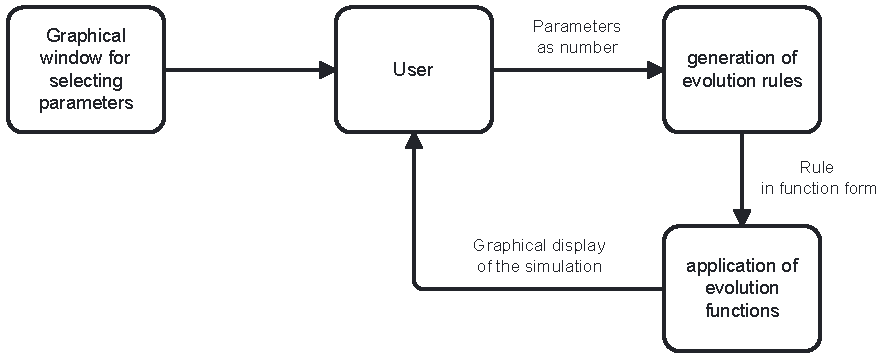
\includegraphics[width=0.9\textwidth]{SystemContext.pdf}
\caption{System Context}
\label{Fig_SystemContext} 
\end{center}
\end{figure}

\begin{itemize}
\item User Responsibilities:
\begin{itemize}
\item The user will have no responsibility for the data they transmits to the system since they will be included in a range of values 
that the system will provide him.
\end{itemize}
\item \progname{} Responsibilities:
\begin{itemize}
\item Provide the user with a simulation that faithfully matches the data the user has given to the system.
\end{itemize}
\end{itemize}

This software is intended for educational and/or artistic use. 
As such, its components must not be used for uses requiring security or critical requirements.

\subsection{User Characteristics} \label{SecUserCharacteristics}

The user does not need any special knowledge to use the program. 
All useful information will be provided by the graphical window for selecting parameters.

\subsection{System Constraints}

No system constraints are identified for this project, as long as its requirements are met.

\section{Specific System Description}

This section first presents the problem description, which gives a high-level
view of the problem to be solved.  This is followed by the solution characteristics
specification, which presents the assumptions, theories, definitions and finally
the instance models.

\subsection{Problem Description} \label{Sec_pd}

\progname{} aims to demonstrate the emergence of macroscopic behavior and structure from microscopic generation and evolution rules.

\subsubsection{Terminology and  Definitions}

This subsection provides a list of terms that are used in the subsequent
sections and their meaning, with the purpose of reducing ambiguity and making it
easier to correctly understand the requirements:

\begin{itemize}

\item A cell : A portion of a display area that contains one or more values

\item The grid : A cell grid as small as possible to simulate a continuous space, such as a computer screen with pixel. The dimensions of this grid are as large as desired.

\item Neighbourhood : Area around a cell, consisting of the cells in that area. This area is delimited by a neighbourhood function

\item Neighbourhood function: Function that takes a cell as input and returns the cells in its neighbourhood.

\item Growth function: Function that takes a cell as input and modifies the value(s) contained in the cell based on its neighbourhood.

\item Structure: Finite set of cells in prolonged interaction.

\item Channel: The definition is the same as in the context of digital images. If the cell has 3 independent values, it can be seen as a color, composed of three channels: RBG


\end{itemize}

\subsubsection{Physical System Description} \label{sec_phySystDescrip}

The physical system of \progname{}, as shown in Figure \ref{Fig_SystemContext}, includes the following elements:

\begin{itemize}

\item[PS1 :] Cells

\item[PS2 :] Growth function

\item[PS3 :] Neighbourhood function

\end{itemize}

\subsubsection{Goal Statements}

\noindent Given the input parameters defined in \ref{sec_DataConstraints}, the goal statements are:

\begin{itemize}

\item[GS\refstepcounter{goalnum}\thegoalnum \label{G_GFCT}:] Create the Growth function

\item[GS\refstepcounter{goalnum}\thegoalnum \label{G_meaningfulLabel}:] Create the Neighbourhood function

\item[GS\refstepcounter{goalnum}\thegoalnum \label{G_meaningfulLabel}:] Apply iterative evolution

\item[GS\refstepcounter{goalnum}\thegoalnum \label{G_meaningfulLabel}:] Define interesting evolution

\item[GS\refstepcounter{goalnum}\thegoalnum \label{G_meaningfulLabel}:] Find some interesting evolution

\end{itemize}

\subsection{Solution Characteristics Specification}

The instance models that govern \progname{} are presented in
Subsection~\ref{sec_instance}.  The information to understand the meaning of the
instance models and their derivation is also presented, so that the instance
models can be verified.


\subsubsection{Assumptions} \label{sec_assumpt}

Since the project does not aim to model a physical system by simplifying it, 
no assumptions of physical simplification will be made. Therefore, this section is not relevant.

\subsubsection{Theoretical Models}\label{sec_theoretical}

No additional assumptions will be made to modify the equations used.
As such, the models are described in section 4.2.5. This section is not relevant.

\subsubsection{General Definitions}\label{sec_gendef}

This section collects the laws and equations that will be used in building the
instance models.

~\newline

\noindent
\begin{minipage}{\textwidth}
\renewcommand*{\arraystretch}{1.5}
\begin{tabular}{| p{\colAwidth} | p{\colBwidth}|}
\hline
\rowcolor[gray]{0.9}
Number& GD\refstepcounter{defnum}\thedefnum \label{GAUSS}\\
\hline
Label &\bf Gauss function \\
\hline
% Units&$MLt^{-3}T^0$\\
% \hline
SI Units& N/A\\
\hline
Equation& 
$G(x) = A \exp\left(-\frac{(x - \mu)^2}{2\sigma^2}\right)$\\
\hline
Description & 
This formula will be used for applying the growth and neighbourhood function on a cell. \\
\hline
  Source & \url{https://en.wikipedia.org/wiki/Gaussian_function} \\
  \hline
  Ref.\ By & None\\
  \hline
\end{tabular}
\end{minipage}\\

~\newline

\noindent
\begin{minipage}{\textwidth}
\renewcommand*{\arraystretch}{1.5}
\begin{tabular}{| p{\colAwidth} | p{\colBwidth}|}
\hline
\rowcolor[gray]{0.9}
Number& GD\refstepcounter{defnum}\thedefnum \label{LO}\\
\hline
Label &\bf Laplacian Operator \\
\hline
% Units&$MLt^{-3}T^0$\\
% \hline
SI Units& N/A\\
\hline
Equation& 
$\nabla^2 u_{i,j} = u_{i+1,j} + u_{i-1,j} + u_{i,j+1} + u_{i,j-1} - 4u_{i,j}$\\
\hline
Description & 
This formula is the discrete approximation of the second derivative. This model models the interactions between two concentration values. It will be used only if the simulation includes multiple channels.\\
\hline
  Source & \url{https://en.wikipedia.org/wiki/Finite_difference#Multivariate_finite_differences} \\
  \hline
  Ref.\ By & None\\
  \hline
\end{tabular}
\end{minipage}\\

~\newline

\noindent
\begin{minipage}{\textwidth}
\renewcommand*{\arraystretch}{1.5}
\begin{tabular}{| p{\colAwidth} | p{\colBwidth}|}
\hline
\rowcolor[gray]{0.9}
Number& GD\refstepcounter{defnum}\thedefnum \label{NL}\\
\hline
Label &\bf Reaction-Diffusion equation \\
\hline
% Units&$MLt^{-3}T^0$\\
% \hline
SI Units& N/A\\
\hline
Equation& 
$\frac{\partial u}{\partial t} = D_u \nabla^2 u + f(u, v)$
 \\
\hline
Description & This model models the interactions between two concentration values. 
It will be used only if the simulation includes multiple channels.\\

\hline
  Source & \url{https://www.karlsims.com/rd.html} \\
  \hline
  Ref.\ By & None\\
  \hline
\end{tabular}
\end{minipage}\\

\subsubsection{Data Definitions}\label{sec_datadef}

\noindent
\begin{minipage}{\textwidth}
\renewcommand*{\arraystretch}{1.5}
\begin{tabular}{| p{\colAwidth} | p{\colBwidth}|}
  \hline
  \rowcolor[gray]{0.9}
  Number& DD\refstepcounter{datadefnum}\thedatadefnum \label{concentration}\\
  \hline
  Label& \bf Concentration \\
  \hline
  Symbol & $u_t$\\
  \hline
  SI Units &  \\
  \hline
  Description& The concentration of species $u$ in a given cell, at a given time $t$.  \\
  \hline
  Sources&  \\
  \hline
  Ref.\ By & \iref{GFCT}, \iref{REDI} \\
  \hline
\end{tabular}
\end{minipage}\\

\subsubsection{Instance Models} \label{sec_instance}    

This section transforms the problem defined in Section~\ref{Sec_pd} into 
one which is expressed in mathematical terms. It uses concrete symbols defined 
in Section~\ref{sec_datadef} to replace the abstract symbols in the models 
identified in Sections~\ref{sec_theoretical} and~\ref{sec_gendef}.
The goal \gsref{G_GFCT} are solved by \iref{GFCT}.

~\newline

%Instance Model 1

\noindent
\begin{minipage}{\textwidth}
\renewcommand*{\arraystretch}{1.5}
\begin{tabular}{| p{\colAwidth} | p{\colBwidth}|}
  \hline
  \rowcolor[gray]{0.9}
  Number& IM\refstepcounter{instnum}\theinstnum \label{REDI}\\
  \hline
  Label& \bf Reaction Diffusion \\
  \hline
  Input& $D_u$,$D_v$, $u_t$, $v_t$, $F$, $k$\\
  \hline
  Output& $u_{t+1} = D_u \nabla^2 u_t - u_t \cdot v_t^2 + F(1 - u_t)$ \\
  &       $v_{t+1} = D_v \nabla^2 v_t + u_t \cdot v_t^2 - (F + k)v_t$ \\
  \hline
  Description&$D_u$ and $D_v$ are the diffusion rate for $u$ and $v$.\\
  & $u_t$ and $v_t$ are the concentrations of elements $u$ and $v$ at time $t$\\
  & We will use the Gray-Scott model to implement the diffusion reaction.
  \\
  \hline
  Sources& https://www.karlsims.com/rd.html \\
  \hline
  Ref.\ By & None\\
  \hline
\end{tabular}
\end{minipage}\\

~\newline

\noindent
\begin{minipage}{\textwidth}
\renewcommand*{\arraystretch}{1.5}
\begin{tabular}{| p{\colAwidth} | p{\colBwidth}|}
  \hline
  \rowcolor[gray]{0.9}
  Number& IM\refstepcounter{instnum}\theinstnum \label{GFCT}\\
  \hline
  Label& \bf Growth function \\
  \hline
  Input& $u_t$, $\alpha$, $\beta$\\
  \hline
  Output& $ u_{t+1} = -1 + 2 \exp \left(-(\frac{u_t - \alpha}{\beta})^2\right)$ \\
  \hline
  Description& We'll use a Gaussian function to start. We want an amplitude between -1 and 1 to simplify the calculations.  \\
  \hline
  Sources&  None \\
  \hline
  Ref.\ By & None\\
  \hline
\end{tabular}
\end{minipage}\\

\subsubsection{Input Data Constraints} \label{sec_DataConstraints}    

Constraints on the input data will be set by the program itself, via a selection interface. The input parameters are decimal numbers whose precision and limits will be determined in a future version of the document.


\subsubsection{Properties of a Correct Solution} \label{sec_CorrectSolution}

This program does not provide a ``solution'', but a visualization of the events induced by the parameter choices made by the user. This section is not relevant.

\section{Requirements}

This section provides the functional requirements, the business tasks that the
software is expected to complete, and the nonfunctional requirements, the
qualities that the software is expected to exhibit.

\subsection{Functional Requirements}

\noindent \begin{itemize}

\item[R\refstepcounter{reqnum}\thereqnum \label{R_Inputs}:] The system shall accept input data from the user before the simulation starts

\item[R\refstepcounter{reqnum}\thereqnum \label{R_Inputs}:] The system must allow modification of input data during simulation

\item[R\refstepcounter{reqnum}\thereqnum \label{R_Selection}:] The parameter selection interface graphically displays the impact of the entered values on the functions used by the simulation.

\item[R\refstepcounter{reqnum}\thereqnum \label{R_Calculate}:] The program must calculate step by step the results of applying the growth function to each cell.

\item[R\refstepcounter{reqnum}\thereqnum \label{R_Output}:] The output should allow the user to correctly distinguish between concentrations of value.

\end{itemize}

\subsection{Nonfunctional Requirements}

\noindent \begin{itemize}

\item[NFR\refstepcounter{nfrnum}\thenfrnum \label{NFR_Accuracy}:]
  \textbf{Accuracy} The accuracy of the simulation must be such that no display inaccuracy can be detected.

\item[NFR\refstepcounter{nfrnum}\thenfrnum \label{NFR_Usability}:] \textbf{Usability} All users should be able to use this software easily.

\item[NFR\refstepcounter{nfrnum}\thenfrnum \label{NFR_Maintainability}:]
  \textbf{Maintainability} The effort required to make any of the likely
    changes listed for \progname{} should be less than $\epsilon$ of the original
    development time.

\item[NFR\refstepcounter{nfrnum}\thenfrnum \label{NFR_Portability}:]
  \textbf{Portability} This program should run on all operating systems supported by the libraries used.

\end{itemize}

\subsection{Rationale}

It is clear that significant mathematical and physics skills are required to simulate a biologically accurate cellular automaton development environment. 
Not having such skills, I limit myself to a basic but correct and useful implementation of a cellular automaton simulation.

\section{Likely Changes}    

\noindent \begin{itemize}

\item[LC\refstepcounter{lcnum}\thelcnum\label{LC_meaningfulLabel}:] Implementing multiple value channels

\item[LC\refstepcounter{lcnum}\thelcnum\label{LC_meaningfulLabel}:] Stochastic equation implementation for the evolution rules
\end{itemize}

\section{Unlikely Changes}    

None

\section{Traceability Matrices and Graphs}

The purpose of the traceability matrices is to provide easy references on what
has to be additionally modified if a certain component is changed.  Every time a
component is changed, the items in the column of that component that are marked
with an ``X'' may have to be modified as well.  Table~\ref{Table:trace} shows the
dependencies of  general definitions and instance models with each other. 
Table~\ref{Table:R_trace} shows the dependencies of instance models and requirements on each other. 

\begin{table}[h!]
\centering
\begin{tabular}{|c|c|c|}
\hline        
	& \dref{GAUSS} & \dref{LO} \\
\hline
\iref{GFCT} & X &  \\ \hline
\iref{REDI} &   & X \\
\hline
\end{tabular}
\caption{Traceability Matrix Showing the Connections Between Items of Different Sections}
\label{Table:trace}
\end{table}

\begin{table}[h!]
\centering
\begin{tabular}{|c|c|c|}
\hline
	& \iref{GFCT} & \iref{REDI} \\
\hline
\rref{R_Calculate}   & X & X \\ 
\hline
\end{tabular}
\caption{Traceability Matrix Showing the Connections Between Requirements and Instance Models}
\label{Table:R_trace}
\end{table}

\section{Values of Auxiliary Constants}

\begin{table}[h!]
  \centering
  \begin{tabular}{|c|c|}
  \hline
  Auxiliary Constants & Values \\
  \hline
  $\epsilon$  & $\frac{1}{20}$ \\ 
  \hline
  \end{tabular}
  \label{Table:Values}
  \end{table}


\end{document}